%-----------------------------------------------------------------------------
%
%               Template for sigplanconf LaTeX Class
%
% Name:         sigplanconf-template.tex
%
% Purpose:      A template for sigplanconf.cls, which is a LaTeX 2e class
%               file for SIGPLAN conference proceedings.
%
% Guide:        Refer to "Author's Guide to the ACM SIGPLAN Class,"
%               sigplanconf-guide.pdf
%
% Author:       Paul C. Anagnostopoulos
%               Windfall Software
%               978 371-2316
%               paul@windfall.com
%
% Created:      15 February 2005
%
%-----------------------------------------------------------------------------


\documentclass{sigplanconf}

% The following \documentclass options may be useful:
%
% 10pt          To set in 10-point type instead of 9-point.
% 11pt          To set in 11-point type instead of 9-point.
% authoryear    To obtain author/year citation style instead of numeric.

\usepackage{amsmath}
\usepackage[pdftex]{graphicx}

\begin{document}

\conferenceinfo{WXYZ '05}{date, City.} 
\copyrightyear{2011} 
\copyrightdata{[to be supplied]} 

\titlebanner{banner above paper title}        % These are ignored unless
\preprintfooter{short description of paper}   % 'preprint' option specified.

\title{Python to Assembly Compilation}
\subtitle{With Reference Counting Garbage Collection}

\authorinfo{Brent Smith}
           {University of Colorado, Boulder}
           {brent.m.smith@colorado.edu}
\authorinfo{Robert Elsner}
           {University of Colorado, Boulder}
           {robert.elsner@colorado.edu}

\maketitle

\begin{abstract}
Integrating a modern dynamic language in to existing systems-level languages (Assembly or C) easily has a number of challenges.  This paper will focus on automatic garbage collection within a subset of the Python language, to enable a Python-like program the ability to cleanly interact with Assembly or C routines without extra intervention from the software developer.  This paper will focus on reference counting garbage collection at the compiler level, to enable automatically freeing no-longer-referenced objects at the end of their useful lifetime.  We will also outline the analysis steps required in the compiler which enable reference tracking, how the abstract syntax tree of the program is altered and what trade-offs are made with such altercations.
\end{abstract}

\category{D.1.5}{Programming Techniques}{Object-oriented Programming}
\category{D.3.3}{Programming Languages}{Language Constructs And Features-Dynamic Storage Management}
\category{D.3.4}{Programming Languages}{Processors-Memory Management (garbage collection)}
\category{D.4.2}{Operating Systems}{Storage Management-Garbage collection}

\terms
Management, Performance, Design, Languages, Algorithms

\keywords
memory management, garbage collection, reference counting, compilation, compilers, programming languages

\section{Introduction}

Python is a modern high level language which has a reference counting garbage collector at its core.  It is also, by default, an interpreted language.  In many cases the usefulness of Python as a productive language is highly desired and a trade-off is made in terms of performance.  While numerous optimizations have been made to the Python run time there is still a usefulness to compile a high level language directly to machine code.  Most high level languages do not allow for direct memory management, instead leaving allocation and de-allocation of memory to the interpreter and garbage collection process.
There are two main classifications for garbage collectors: generational or tracing collectors and reference-counting collectors.  Generational or tracing collectors make periodic inspection of all objects to determine if they are reachable by a pointer or object reference.  These are the modern batch of garbage collectors and have the best performance 
Given a naive implementation of a direct Python to x86-assembly compiler which disregards all memory management, we explore the choices and consequences of adding a reference counting garbage collector.  Our base Python-like language includes classes, objects, functions, lambdas, simple math, lists, dictionaries and integer primitives.
\subsection{Disadvantages}
In general a reference count garbage collector will have shorter pause times for the garbage collection phase, but will incur a higher performance penalty \cite{joisha}\cite{blackburn}.  Reference-counting collectors have been implemented which defer the de-allocation, called lazy reference-counting, to some later time and some improvements on such strategies have been made \cite{boehm}.  Without extra work a strictly reference-counting collector will leak memory when references contain cycles, and multiple algorithms have been presented as solutions to this problem.
\subsection{Advantages}
One potential advantage that reference-counting garbage collectors have is the ability to be implemented in hardware \cite{joao}.  Given the significant cost of garbage collection \cite{hertz} any hardware assisted acceleration would be highly desirable if it is flexible enough to adapt across multiple garbage collection techniques. 
\par
Real-time systems are rarely implemented in languages which are garbage collected, but reference-counting garbage collection has been adapted to hard real-time systems \cite{?}.  Due to immediate knowledge that an object is no longer in use reference counting garbage collection can allow for destructors or finalizers to be run immediately which can enhance the clean up of system resources.
\section{Implementation}
We develop a base compiler which generates x86 assembly code and then alter the compiler to include reference counting and garbage collection.
\subsection{Language}
A subset of Python has been chosen which includes functions, objects, lambdas, and the primitives integer, boolean.  We implement this as a reference compiler which is extended to include reference counting.  This language has no built in parallelism but Levanoni, et. al. have shown that reference counting is a valid approach for multprocessor systems.\cite{levanoni}
\par
Starting from our reference compiler, we treat any object which is not an integer or boolean primitive as a C structure.  This structure was modified to include a reference counter and in all places where such a structure was allocated we converted the allocation to use a statistics tracking allocator and set the reference count to an initial value of 0.
\par
We chose to implement our own memory routines primarily to investigate object lifetime (initial allocation time and final de-allocation time) as well as allow us the ability to detect memory leaks.  Since every allocation of an object in our language uses this wrapper we know exactly how much memory has been allocated and what objects were never de-allocated.
\par
The basic premise of such routines is to wrap the provided malloc and free, request slightly more memory than required.  That extra memory is what where the reference counter is stored and the pointer location is returned which skips the counter.  The memory routines also create a linked list to track all of the allocations in a structure for statistics gathering and leak detection.
\begin{figure}
\begin{center}
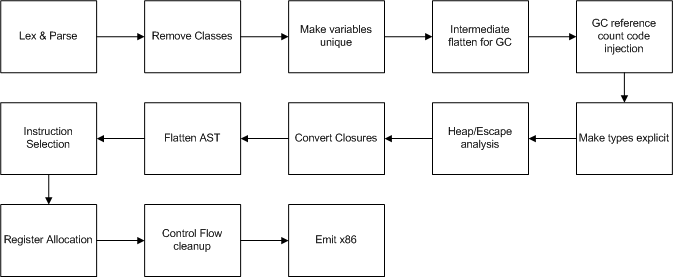
\includegraphics[scale=0.48]{compiler_flow.png}
\end{center}
\caption{Compiler Architecture}
\label{fig-comparch}
\end{figure}

\subsection{Compiler Flow}
Refer to Figure~\ref{fig-comparch} for the compiler data flow.  Each stage operates on an abstract syntax tree, the relevant new stages are the garbage collection flattening stage and the reference count AST transformation stage.

\subsection{Syntax Tree Modifications}
\subsubsection{New compiler stages}
We added two new stages to our reference compiler.  The first stage is a modified flattening stage, which produces a flattened AST to aid in the reference determination.  The next stage is the actual reference determination and AST transformation, where the compiler determines what variables will be objects and when assignments happen and adds appropriate calls to increment and decrement the reference counter of the object as needed.
\par
Our initial assumption was that we could easily add the increment and decrement reference counter operations in the reference compilers flatten stage, however because this stage is after type explication and there are variables created which do not correspond to a type in the language the pre-flatten stage was necessary.  This stage converts all expressions in to assignments to temporary variables.  At this stage we know every expression is operating on types.
\subsubsection{Analysis on when to decrement an object reference}
The next new stage is the reference counting AST transformation.  In this stage we take the flattened tree and look for assignments which are setting list elements, dictionary values, class attributes, object attributes or variables.  The compiler determines what variables are created in the current scope and injects code at the beginning of that scope to set the value initially.  We decided on this approach to simplify determining when an object is first assigned and this allows us to simply decrement the reference counter to the object before an assign, regardless of the variables state.
\subsubsection{Temporary Variables}
The compiler creates temporary variables in a number of situations (namely function calls and as a result of flattened expressions).  These temporary variables need not hang on to their memory reference past the next assignment to the actual result variable.
\subsection{Runtime Modifications}
Our runtime consisted of C functions which took care of allocating and initializing memory for a new object of a given type.  The obvious modifications included setting the reference counter initially to zero and creating a number of free functions to free each type of object.
\par
In the free\emph{\_type} functions it was necessary to add further calls to decrement the reference counter of any objects referenced by the type.  For a list list we iterate the values contained in the list, decrementing their reference (which can result in freeing that object).  For a dictionary we decrement the reference counter on keys as well as values contained in the dictionary, since both can be objects.
\subsection{Interesting Problems}
We encountered a number of interesting questions during this implementation and summarize them below.
\subsubsection{Addition of Lists}
In the current runtime an entirely new list is created when two lists are added together.  At the assignment level our compiler can determine (due to the flattened structure) that the left-hand-side and the right-hand-side of the addition need their reference counters manipulated, however the assignment from an addition to a list creates an entirely new list which should properly increment the reference counter to all objects in both lists.
\subsubsection{Variable Assignment}
We wanted a simple way to determine when to decrement an objects reference counter.  Our first implementation was to add a call to decrement the counter before every assignment.  However, because a variable can be created at any point in program execution we couldn't just blindly decrement the counter of an object since the variable will be uninitialized, and could be pointing at memory that makes it look like an object or accidentally references an object.
\par
The solution we took makes a slight modification to program behaviour, but we feel it is an acceptable trade-off.  In every scope, we add an immediate assignment as the first instructions.  This assignment is to a primitive, so it costs us no memory and then a decrement on the reference counter amounts to a function call with a no-op.  This function call overhead could potentially be avoided by adding code to check if the variable points to an object or a primitive and is a future enhancement for performance.
\par
An additional problem is lack of static single assignment.  When a variable is re-assigned to its own name, the code should decrement the reference counter on the previous version of the object and increment it on the new version.
\subsection{Assembly Output}
We modified the x86 assembly to include calls to set up our memory tracking system and print statistics at the end of the program.
\section{Results}
\subsection{Execution}
\subsection{Memory}
\section{Future work}
\section{Related Work}
\appendix
\section{Appendix Title}

This is the text of the appendix, if you need one.

\acks

We would like to thank Jeremy Siek and Evan Chang for the course notes from which the compiler design is derived.

% We recommend abbrvnat bibliography style.

\bibliographystyle{abbrvnat}

% The bibliography should be embedded for final submission.

\begin{thebibliography}{}
\softraggedright
\bibitem{joisha}
Pramod G. Joisha. 2006. Compiler optimizations for nondeferred reference: counting garbage collection. In Proceedings of the 5th international symposium on Memory management (ISMM '06). ACM, New York, NY, USA, 150-161. DOI=10.1145/1133956.1133976

\bibitem{blackburn}
Stephen M. Blackburn and Kathryn S. McKinley. 2003. Ulterior reference counting: fast garbage collection without a long wait. In Proceedings of the 18th annual ACM SIGPLAN conference on Object-oriented programing, systems, languages, and applications (OOPSLA '03). ACM, New York, NY, USA, 344-358. DOI=10.1145/949305.949336

\bibitem{boehm}
Hans-J. Boehm. 2004. The space cost of lazy reference counting. In Proceedings of the 31st ACM SIGPLAN-SIGACT symposium on Principles of programming languages (POPL '04). ACM, New York, NY, USA, 210-219. DOI=10.1145/964001.964019 

\bibitem{joao}
José A. Joao, Onur Mutlu, and Yale N. Patt. 2009. Flexible reference-counting-based hardware acceleration for garbage collection. In Proceedings of the 36th annual international symposium on Computer architecture (ISCA '09). ACM, New York, NY, USA, 418-428. DOI=10.1145/1555754.1555806

\bibitem{hertz}
Matthew Hertz and Emery D. Berger. 2005. Quantifying the performance of garbage collection vs. explicit memory management. In Proceedings of the 20th annual ACM SIGPLAN conference on Object-oriented programming, systems, languages, and applications (OOPSLA '05). ACM, New York, NY, USA, 313-326. DOI=10.1145/1094811.1094836  

\bibitem{levanoni}
Yossi Levanoni and Erez Petrank. 2006. An on-the-fly reference-counting garbage collector for java. ACM Trans. Program. Lang. Syst. 28, 1 (January 2006), 1-69. DOI=10.1145/1111596.1111597 

\end{thebibliography}

\end{document}
